% =====================================================================================================
\section{Hardware Results}\label{sec:hwresults}
\subsection{Cycles and throughput}
% generated by paper/make_assets.py from paper/data -- do not edit
\begin{table}[t]
\caption{Encoder cycles per frame in RTL simulation (160x128, 100\,MHz). The last column extrapolates to 640$\times$480 at the same cycles per pixel.}
\label{tab:cycles}
\centering\small
\resizebox{\columnwidth}{!}{%
\begin{tabular}{lrrrr}
\toprule
Mode & Cycles & Cycles/pixel & $\Delta$ vs E0 & fps (640$\times$480) \\
\midrule
E0 & 33515 & 1.636 & +0 & 199 \\
E1 & 33517 & 1.637 & +2 & 199 \\
E2 & 33513 & 1.636 & -2 & 199 \\
E3 & 33517 & 1.637 & +2 & 199 \\
E4 & 33510 & 1.636 & -5 & 199 \\
\bottomrule
\end{tabular}}
\end{table}

In RTL simulation of a 160$\times$128 frame, the cycle counts of E0--E4 differ by at most \MaxExtraCycles{} cycles (Table~\ref{tab:cycles}), which is handshake noise rather than encryption work: as Proposition~\ref{prop:supply} predicts, encryption costs no cycles. Above the floor of 1.5 cycles per pixel, the only cost is filling the first MCU row: on \NumScaleSizes{} frame sizes the RTL follows~\eqref{eq:fill}, \CyclesPerPixel{} cycles per pixel at 160$\times$128 and \CppVGA{} at 640$\times$480 (Fig.~\ref{fig:throughput}).

\begin{figure}[t]
\centering
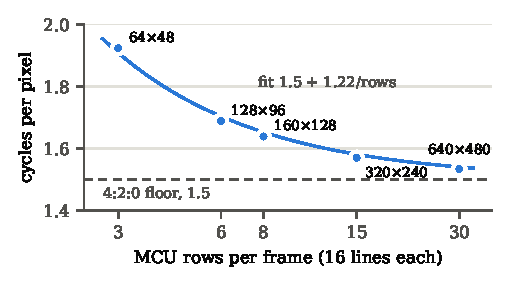
\includegraphics[width=\columnwidth]{figures/fig_throughput.pdf}
\caption{Cycles per pixel of the encoder RTL against frame height, measured in cycle-accurate simulation (dots), with the fitted law $1.5+\FillA/r$ of~\eqref{eq:fill} for $r$ MCU rows.}
\label{fig:throughput}
\end{figure}

\begin{figure}[t]
\centering
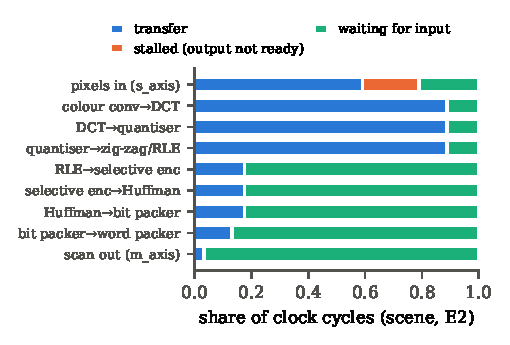
\includegraphics[width=\columnwidth]{figures/fig_stall.pdf}
\caption{Where the clock cycles go: share of cycles in which each handshake of the encoder pipeline transfers data, is stalled by its consumer, or waits for its producer (RTL simulation, synthetic scene, E2). Everything after the run-length coder, including the cipher, idles most of the time.}
\label{fig:stall}
\end{figure}
\textit{Where the cycles go.} Monitoring every handshake of the RTL pipeline over \ProfileCases{} cases (three images, three levels) shows the same cycles per pixel to within \ProfileCppSpread{} for every image and level, and an entropy path (run-length coding, encryption, Huffman coding, packing) that waits for data at least \EntropyIdle\,\% of the time (Fig.~\ref{fig:stall}). Faster designs must therefore widen the transform path, not the cipher, which is what the lanes do.

\textit{Lanes.} Measured at 100\,MHz on 640$\times$480 frames, bit-exact for every frame (Fig.~\ref{fig:lanesrtl}), one, two and four lanes reach \RtlOneLaneMpix, \RtlTwoLanesMpix{} and \RtlFourLanesMpix\,Mpixel/s (\RtlOneLaneCpp, \RtlTwoLanesCpp{} and \RtlFourLanesCpp{} cycles per pixel), against the bounds \BoundOneMpix, \BoundTwoMpix{} and \BoundFourMpix{} of~\eqref{eq:lanes}. Four lanes give \RtlFourLanesSpeedup$\times$ the single pipeline, \RtlFourLanesFps{} frames/s at 640$\times$480 or \RtlFourLanesHdFps{} at 1080p, above the \mbox{150\,Mpixel/s} that the commercial encoder of~\cite{logijpge} reports at 150\,MHz without any cryptography, at two thirds of its clock. The gap to the bound has two causes: a frame starts only after the previous one is done, so every frame pays~\eqref{eq:fill} once, and each segment adds a keystream restart and a byte flush. An event model that also lets the next frame's first MCU row arrive early projects \ProjTwoLanesMpix{} and \ProjFourLanesMpix\,Mpixel/s (Fig.~\ref{fig:lanes}). The latency from the first pixel to the first scan word is \RtlFourLanesLatUs\,$\mu$s (\RtlFourLanesLatLines{} lines of a 640$\times$480 frame) for any number of lanes: the 16 lines of the first MCU row plus the pipeline. E5, with one restart per MCU, costs a few per cent of throughput in the lane encoder. Two build options trade along other axes. With camera-native YUYV input (four pixels per beat, Section~\ref{sec:lanes}) four lanes reach \YuyvFourLanesMpix\,Mpixel/s (\YuyvFourLanesCpp{} cycles per pixel) and read \YuyvFourLanesInMBs\,MB/s from DDR instead of \RtlFourLanesInMBs; with one line-buffer set per lane instead of two, four lanes keep \NbufOneFourLanesMpix\,Mpixel/s (\NbufOneFourLanesCpp{} cycles per pixel) on half the converter memory, which is what lets four lanes take 1080p lines on this device.

\begin{figure}[t]
\centering
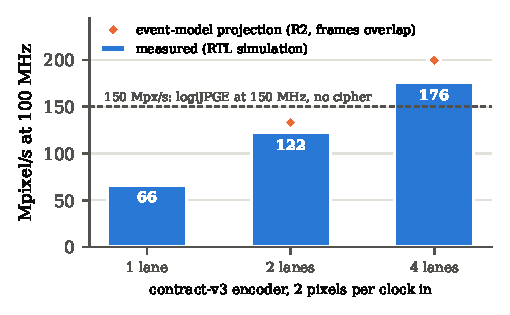
\includegraphics[width=\columnwidth]{figures/fig_lanes_rtl.pdf}
\caption{Throughput of the lane encoder, 640$\times$480 frames at 100\,MHz, measured in cycle-accurate simulation with every frame bit-exact against the golden model (bars), next to the event-model projection with overlapping frames (diamonds) and the published figure of a commercial encoder without cryptography~\cite{logijpge} (dashed).}
\label{fig:lanesrtl}
\end{figure}
\begin{figure}[t]
\centering
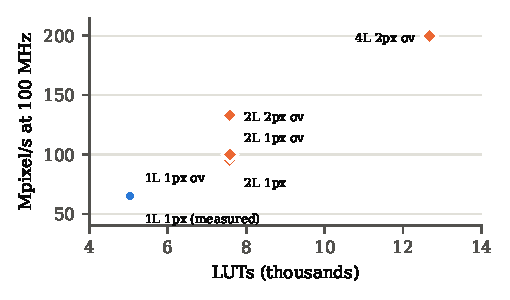
\includegraphics[width=\columnwidth]{figures/fig_lanes.pdf}
\caption{Projected throughput at 100\,MHz against LUTs for 640$\times$480 frames (event model calibrated on the measured RTL law). Labels: $L$ lanes, pixels per clock at the input, ``ov'': the next frame overlaps the current one; the circle is the measured single pipeline.}
\label{fig:lanes}
\end{figure}

\subsection{Area, timing and power}
% generated by paper/make_assets.py from paper/data -- do not edit
\begin{table}[t]
\caption{Resources on the xc7z020 (53\,200 LUT, 106\,400 FF, 140 BRAM36, 220 DSP). Source: Vivado post-route, out of context, 100\,MHz with I/O delays of 20\,\% of the period, WNS +0.630\,ns.}
\label{tab:resources}
\centering\small
\resizebox{\columnwidth}{!}{%
\begin{tabular}{lrrrr}
\toprule
Block & LUT & FF & BRAM36 & DSP \\
\midrule
Encoder (all) & 4785 (9.0\%) & 3051 (2.9\%) & 25.5 (18.2\%) & 23 (10.4\%) \\
\quad colour conversion + line buffers & 459 & 220 & 25 & 0 \\
\quad DCT and quantizer & 806 & 69 & 0 & 22 \\
\quad zig-zag, Huffman, packing & 717 & 323 & 0 & 0 \\
\quad keystream generator (Ascon) & 949 & 851 & 0 & 0 \\
\quad tag unit (Ascon) & 1358 & 1072 & 0 & 0 \\
\quad selective encryption & 82 & 24 & 0 & 0 \\
\quad AXI-Lite registers & 392 & 451 & 0 & 0 \\
\bottomrule
\end{tabular}}
\end{table}

After place and route in Vivado the single-pipeline encoder meets \TopMhz\,MHz on the xc7z020 (WNS $+$\TopWns\,ns, out of context, I/O delays of 20\,\% of the period), i.e.\ \TopMpix\,Mpixel/s or \FpsVGA{} frames/s at 640$\times$480. Table~\ref{tab:resources} gives the resources (\TopLuts{} LUTs, \TopLutPct\,\% of the device). The two Ascon instances take \CryptoLutShare\,\% of the LUTs; the selective-encryption stage itself is tiny; all \ConvBram{} BRAM36 are the converter's line buffers for 2048-pixel lines. With switching activity from simulating a real frame (SAIF), the encoder draws about \SaifTopMw\,mW; the vectorless estimate is \TopPowerMw\,mW. Two lanes take \TwoLanesLuts{} LUTs, \TwoLanesBram{} BRAM36 and \TwoLanesDsp{} DSPs (WNS $\TwoLanesWns$\,ns), four lanes \FourLanesLuts{} LUTs, \FourLanesBram{} BRAM36 and \FourLanesDsp{} DSPs (WNS $\FourLanesWns$\,ns, lines up to 1024 pixels). E5 adds no BRAM or DSP; with two lanes it draws \SaifLanesEfiveMw\,mW against \SaifLanesEtwoMw\,mW for E2. Out of context the single pipeline and two lanes also meet 125\,MHz (WNS \TopWnsAtOneTwoFive{} and \LanesTwoWnsAtOneTwoFive\,ns, Section~\ref{sec:hardware}). All three complete PYNQ-Z2 systems close timing at 100\,MHz: the single pipeline with \OverlayLuts{} LUTs (WNS $\OverlayWns$\,ns), two lanes on a 64-bit pixel stream with \OverlayLanesLuts{} LUTs (WNS $\OverlayLanesWns$\,ns), and four lanes with \OverlayLanesFourLuts{} LUTs, \OverlayLanesFourBram{} BRAM36 and \OverlayLanesFourDsp{} DSPs (WNS $\OverlayLanesFourWns$\,ns, \OverlayLanesFourLutPct\,\% of the LUTs); Vivado estimates \OverlayPowerW, \OverlayLanesPowerW{} and \OverlayLanesFourPowerW\,W for the complete systems, dominated by the processing system.

% generated by paper/make_assets.py from paper/data -- do not edit
\begin{table}[t]
\caption{Comparison with published FPGA designs. Their numbers are as reported by each source; ours are
post-route (Table~\ref{tab:resources}) with throughput from the RTL cycle count. Mpx/s: million pixels per second.}
\label{tab:compare}
\centering\small
\resizebox{\columnwidth}{!}{%
\begin{tabular}{llrrrrrl}
\toprule
Design & Device & LUT & BRAM & DSP & MHz & Mpx/s & Crypto \\
\midrule
Ours: encoder & Zynq-7020 & 5{,}039 & 24.5 & 23 & 100 & 61 & sel.\ AEAD \\
Ours: one Ascon & Zynq-7020 & 860--969 & 0 & 0 & 100 & -- & AEAD core \\
logiJPGE~\cite{logijpge} & Zynq-7020 & 3{,}240 & 16 & 30 & 150 & 150 & none \\
CAST JPEG-E-S~\cite{castjpeg} & Artix-7 & 3{,}069 & 2 & 16 & 166 & -- & none \\
Khairallah~\cite{khairallah2023} & Artix-7 & 1{,}031 & 0 & 0 & 200 & -- & MAC \\
Kurian~\cite{kurian2025} & Artix-7 & 5{,}335 & 32 & 0 & 100 & -- & AEAD \\
\bottomrule
\end{tabular}}
\end{table}

% generated by paper/make_assets.py from paper/data -- do not edit
\begin{table}[t]
\caption{Hardware figures of merit at 100\,MHz, 640$\times$480, E2: throughput from cycle-accurate RTL simulation (no DMA stalls), area and power post-route. Energy per pixel = on-chip power / throughput.}
\label{tab:hweff}
\centering\small\setlength{\tabcolsep}{2.5pt}
\resizebox{\columnwidth}{!}{%
\resizebox{\columnwidth}{!}{%
\begin{tabular}{lrrrrrrr}
\toprule
Design & LUT & Mpx/s & Mpx/s per kLUT & Gbit/s in & fps 1080p & Power (mW) & nJ/pixel \\
\midrule
Ours{,} single pipeline (v2) & 5{,}037 & 65 & 12.9 & 1.56 & 31 & 210 (SAIF) & 3.22 \\
Ours{,} 2 lanes & 10{,}069 & 122 & 12.1 & 2.94 & 59 & 319 (SAIF) & 2.61 \\
Ours{,} 4 lanes & 16{,}893 & 176 & 10.4 & 4.22 & 85 & 555 (vectorless) & 3.16 \\
\bottomrule
\end{tabular}}}
\end{table}


\subsection{Comparison}
Table~\ref{tab:compare} sets the design against published FPGA work. Each of our Ascon cores (\AsconLutMin--\AsconLutMax{} LUTs) is as small as the round-per-cycle Ascon-p cores of~\cite{khairallah2023}; our JPEG datapath without the cipher (colour conversion, transform, quantizer and entropy coder in Table~\ref{tab:resources}) uses fewer LUTs than the commercial encoders~\cite{logijpge,castjpeg}, which however process one sample per clock at 150--166\,MHz with less block RAM and no cryptography. Table~\ref{tab:hweff} gives the figures of merit that hardware papers compare: \HeTopPerKlut, \HeTwoPerKlut{} and \HeFourPerKlut\,Mpixel/s per thousand LUTs for one, two and four lanes, against \HeKishorePerKlut{} for the scrambling encoder of Kishore et al.~\cite{kishore2015} and \HeLogiPerKlut{} for the commercial encoder without cryptography~\cite{logijpge}; and \HeTopNj, \HeTwoNj{} and \HeFourNj\,nJ per pixel. One Ascon core accepts a 128-bit block every \AsconCyclesPerBlock{} clocks once initialized (eight rounds and one handshake, measured in RTL), i.e.\ \AsconGbps\,Gbit/s at 100\,MHz or \AsconGbpsPerKlut\,Gbit/s per thousand LUTs of the larger instance; the selective encryption needs far less, since it consumes at most one sign bit and the amplitude bits of each non-zero coefficient. The lanes buy throughput, not efficiency: each lane carries its own transform and line buffers, so area grows with $L$ while the energy per pixel stays roughly constant.

\subsection{Board evaluation}\label{sec:board}
% generated by paper/make_assets.py from paper/data -- do not edit
\begin{table*}[t]
\caption{On the PYNQ-Z2 (24 Oct 2026): the final board images, each at the clock it was built for, and the same
function on the board's ARM Cortex-A9. Bit-exact: every frame of every level compared byte for byte (scan and tag)
with the golden model running on the board (58 frames in all). Fabric: START to DONE from
the encoder's CYCLES register for one 640$\times$480 frame (Mpixel/s in brackets); wait: share of those cycles in
which the encoder could take a pixel but the DMA had none, mostly because the Python driver starts the DMA after the encoder. Frame: a complete authenticated JPEG with headers (and
for E5 the segment order) on the ARM, the pixels already in the DMA buffer as a camera would leave them, median of
50 frames (frames/s in brackets). ARM rows: median of 30 frames; ``file'' encrypts the whole JPEG, so it does not
play without the key.}
\label{tab:board}
\centering\small\setlength{\tabcolsep}{4pt}
\resizebox{\textwidth}{!}{%
\begin{tabular}{lrlrrrr}
\toprule
Encoder & MHz & Bit-exact & Fabric, ms & Wait (\%) & E2 frame, ms & E5 frame, ms \\
\midrule
4 lanes & 125 & E0--E5 & 1.97 (156) & 31 & 5.9 (169) & 8.4 (119) \\
2 lanes & 100 & E0--E5 & 3.06 (100) & 21 & 7.0 (144) & 9.8 (102) \\
1 lane & 100 & E0--E4 & 5.34 (58) & 12 & 9.2 (108) & -- \\
\midrule
ARM, ours in C, 1 core & -- & E0--E5 & -- & -- & 114.2 (8.8) & 133.0 (7.5) \\
ARM, ours in C, 2 cores & -- & E0--E5 & -- & -- & 61.6 (16.2) & 74.8 (13.4) \\
ARM, libjpeg-turbo, no security & -- & -- & -- & -- & 28.8 (34.8) & -- \\
ARM, libjpeg-turbo + Ascon (file) & -- & -- & -- & -- & 31.7 (31.5) & -- \\
ARM, libjpeg-turbo + AES-GCM (file) & -- & -- & -- & -- & 31.9 (31.3) & -- \\
\bottomrule
\end{tabular}}
\end{table*}

Following the practice of Section~\ref{sec:evalpractice}, the board evaluation on the PYNQ-Z2 has four parts, all scripted and rehearsed against an emulation of the bitstream: (A1) a bit-exact gate that encodes frames of two sizes in every level on the fabric and compares every byte and tag with the golden model; (A2) the encode time with registers and DMA, and the full frame time including the ARM's headers; (A3) the same function on the board's processing system: our encoder compiled in C for the Cortex-A9, gated bit-exact against the golden model in every level and run on one and both cores (contract-v3 segments are independent, so the two cores act like two lanes), next to libjpeg-turbo alone and with whole-file Ascon-AEAD128 or AES-GCM, the fair baseline because that core has no AES instructions; and (A4) power from an inline meter, idle and under each workload, giving energy per frame. Parts A1 and A2 are done (Table~\ref{tab:board}). The two-lane E5 bitstream, rebuilt after one defect in the block design (the DMA's write master was left unconnected; Table~\ref{tab:bugs} lists the lesson), is bit-exact with the golden model in every level \BoardModes{} at \BoardSizes{}: \BoardFramesTotal{} frames, every scan byte and every tag. The board thus confirms Lemma~\ref{lem:format} and the lane, E5 and tag logic on silicon, not only in simulation. With our Python driver a 640$\times$480 frame takes \BoardMsVGA\,ms (\BoardFpsVGA{} frames/s; \BoardFpsQVGA{} at 320$\times$240), and the times of E0--E4 differ by at most \BoardSpreadMsVGA\,ms: on silicon too, encryption costs no time. That time is dominated by the ARM, which converts and copies every pixel into the DMA buffer and flushes the cache, not by the fabric, which needs \RtlTwoLanesVgaMs\,ms per frame in RTL simulation; E5 adds \BoardEfiveExtraMsVGA\,ms for splitting and reordering the segments on the ARM. The rebuilt bitstream adds three counters to the register map (clocks from start to done, clocks waiting for pixels, clocks stalled by the output DMA), so the fabric-only time is read from the silicon itself, and the driver now writes the pixels straight into the DMA buffer and maintains the cache only over the frame's bytes. \TODO{A2 fabric-only time from the counters and the new driver, A3 PS baseline (future\_work/arm/arm\_baseline.py), A4 measured power and energy per frame.}
